\protect \section *{\protect \nameref  *{Kinematics}}
\begin{Solution}{1.{6}}
		\begin{enumerate}[label = (\alph*)]
			\item Graph $x$ versus $t$ for the range $t = 0$~\si{\second} to $t = 4$~\si{\second}:		
			
			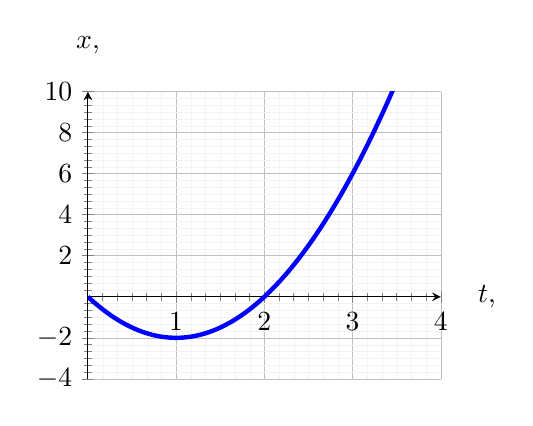
\begin{tikzpicture}
			\begin{axis}[%
			% === Налаштування сітки ===
			grid = both,
			grid style={line width=.1pt, draw=gray!10},
			major grid style={line width=.2pt,draw=gray!50},
			minor tick num = 5,
			minor grid style = {line width=.1pt,draw=gray!10},
			% === Налаштування положення координатних осей ===
			axis lines = middle,
			axis line style={-stealth},
			% === Вибір підписів шкали для відображення ===
			xtick = {0,1,...,4},
			ytick = {-4,-2,...,10},
			% === Підпис координатних осей ===
			xlabel={$t$, \si{\second}},
			ylabel={$x$, \si{\meter}},
			% === Положення підпису координатних осей ===
			xlabel style={right = 10pt},
			ylabel style={above = 10pt},
			% === Налаштування мінімальних та максимальних значень координат ===
			xmin = 0,
			xmax =  4,
			ymin = -4,
			ymax =  10,
			% === Налаштування розміру графіка ===
			width=0.5\linewidth,
			]
			\addplot+[blue, no marks, domain={0:4}, samples=100, ultra thick] {-4*x+2*x^2};
			\end{axis}
			\end{tikzpicture}
			
			\item Displacement of the particle in the time intervals $t = 0$~\si{\second}
			to $t = 1$~\si{\second} is $\Delta x = -2$~\si{\meter},  displacement of the particle in the time intervals $t = 1 $~\si{\second} to $t = 5$~\si{\second} is $\Delta x = + 8$~\si{\meter}.
			\item $\left\langle v\right\rangle  = -2$~\si{\meter\per\second}.
			\item $v_x = 6$~\si{\meter\per\second}.
		\end{enumerate}
	
\end{Solution}
\begin{Solution}{1.{7}}
		\begin{enumerate*}[label = (\alph*)]
			\item $v = \frac{\alpha t^2}{2}$, $a = \frac{\alpha^2}{2}$;
			\item $\left\langle v \right\rangle = \frac{\sqrt{s}}{2}$.
		\end{enumerate*}
	
\end{Solution}
\begin{Solution}{1.{13}}
		$\alpha =69.3^\circ$.
	
\end{Solution}
\begin{Solution}{1.{15}}
		$a = \alpha\sqrt{1 + (4\pi n)^2}$~0.8~m/s\textsuperscript{2}.
	
\end{Solution}
\begin{Solution}{1.{17}}
		$R = \frac{\alpha^3}{2\beta s}$, $a = \alpha\sqrt{1 + \left(\sqrt{\frac{4\beta s^2}{\alpha^3}} \right) }$.
	
\end{Solution}
\begin{Solution}{1.{18}}
		\begin{enumerate*}[label = (\alph*)]
			\item $s = A\omega \tau$,
			\item $\nfrac{\pi}{2}$.
		\end{enumerate*}
	
\end{Solution}
\begin{Solution}{1.{19}}
		$\tan\alpha = \frac{2s}{R}$
	
\end{Solution}
\begin{Solution}{1.{24}}
		\begin{enumerate*}[label = (\alph*)]
		\item $\omega = 8.0$~\si{\radian\per\second}, $\beta = 1.3$~\si{\radian\per\square\second};
		\item $17^\circ$.
		\end{enumerate*}	
	
\end{Solution}
\begin{Solution}{1.{25}}
		\begin{enumerate*}[label = (\alph*)]
			\item $\phi = \frac{\omega_0}{a}(1- e^{-at})$;
			\item $\omega = \omega_0e^{-at}$.
		\end{enumerate*}
	
\end{Solution}
